\documentclass[aspectratio=169]{beamer}
\usetheme{Singapore}
\usecolortheme{default}

% Packages
\usepackage{amsmath, amsfonts, amssymb}
\usepackage{graphicx}
\usepackage{tikz}
\usepackage{pgfplots}
\usepackage{booktabs}
\usepackage{array}
\usepackage{multicol}
\usepackage{hyperref}
\usepackage{float}

\pgfplotsset{compat=1.17}

% Color definitions
\definecolor{kentech_blue}{RGB}{0,51,102}
\definecolor{kentech_orange}{RGB}{255,102,0}
\definecolor{safety_green}{RGB}{34,139,34}
\definecolor{warning_red}{RGB}{220,20,60}

% Custom theme colors
\setbeamercolor{title}{fg=white,bg=kentech_blue}
\setbeamercolor{frametitle}{fg=white,bg=kentech_blue}
\setbeamercolor{structure}{fg=kentech_blue}
\setbeamercolor{block title}{bg=kentech_blue,fg=white}
\setbeamercolor{block body}{bg=kentech_blue!10}

% Title slide information
\title[BAC Prediction Model]{🍺 Blood Alcohol Concentration Prediction Model}
\subtitle{Implementation using Fractional Differential Equations and Mittag-Leffler Functions}
\author[G2 Team]{Hyunjun Jang \and Minyeop Jin \and Sangsu Lee \and Seojin Choi}
\institute[KENTECH]{Korea Institute of Energy Technology (KENTECH)\\
Engineering Mathematics 1 - Group 2}
\date{\today}

% Custom commands
\newcommand{\highlight}[1]{\textcolor{kentech_orange}{\textbf{#1}}}
\newcommand{\safety}[1]{\textcolor{safety_green}{\textbf{#1}}}
\newcommand{\warning}[1]{\textcolor{warning_red}{\textbf{#1}}}

\begin{document}

% Title slide
\begin{frame}
    \titlepage
    \begin{center}
        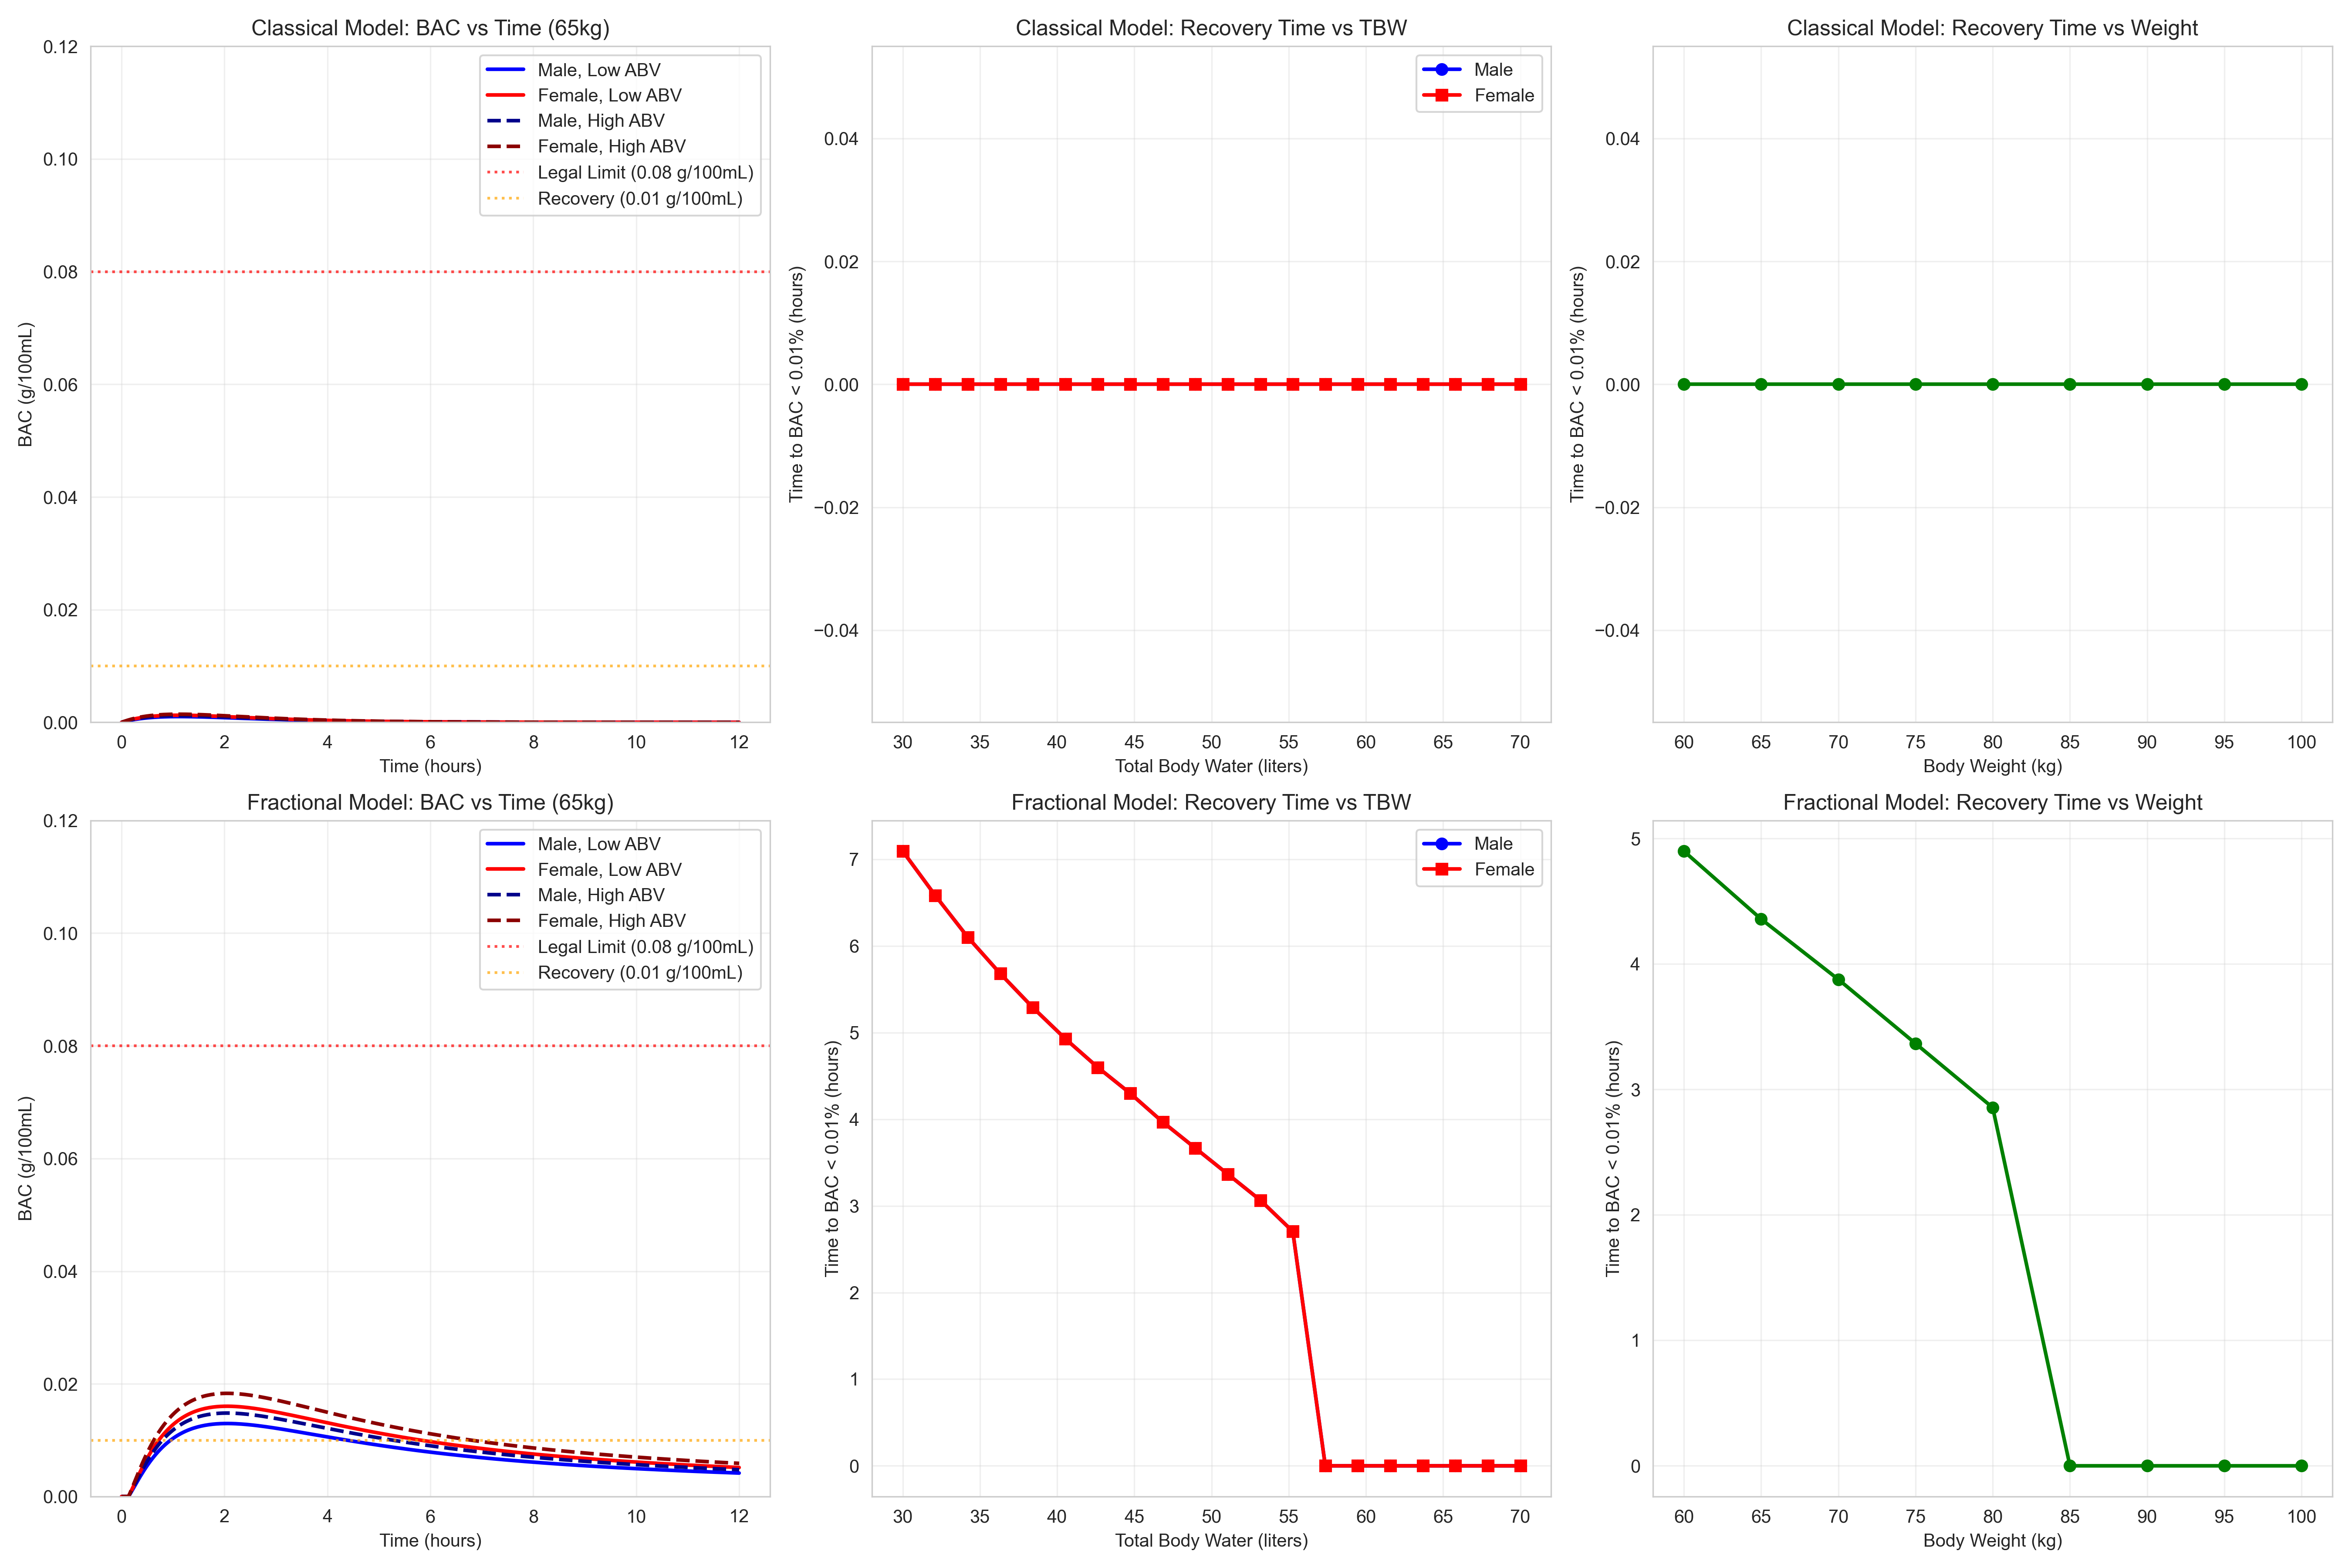
\includegraphics[width=0.15\textwidth]{../bac_comparison.png}
    \end{center}
\end{frame}

% Table of Contents
\begin{frame}{Presentation Overview}
    \tableofcontents
\end{frame}

\section{Introduction \& Problem Statement}

\begin{frame}{Project Motivation}
    \begin{columns}
        \begin{column}{0.6\textwidth}
            \begin{block}{Real-World Problem}
                \begin{itemize}
                    \item \warning{42 drunk driving incidents daily} in South Korea (2019-2023)
                    \item \warning{75,950 alcohol-related accidents} over 5 years
                    \item \warning{1,161 fatalities, 122,566 injuries}
                    \item Peak incidents: Thursday/Friday 10PM-midnight
                \end{itemize}
            \end{block}
            
            \begin{block}{Young Adults' Challenge}
                \begin{itemize}
                    \item Lack of understanding of personal alcohol tolerance
                    \item Trial-and-error approach leads to accidents
                    \item Need for \highlight{scientific prediction method}
                \end{itemize}
            \end{block}
        \end{column}
        
        \begin{column}{0.4\textwidth}
            \begin{center}
                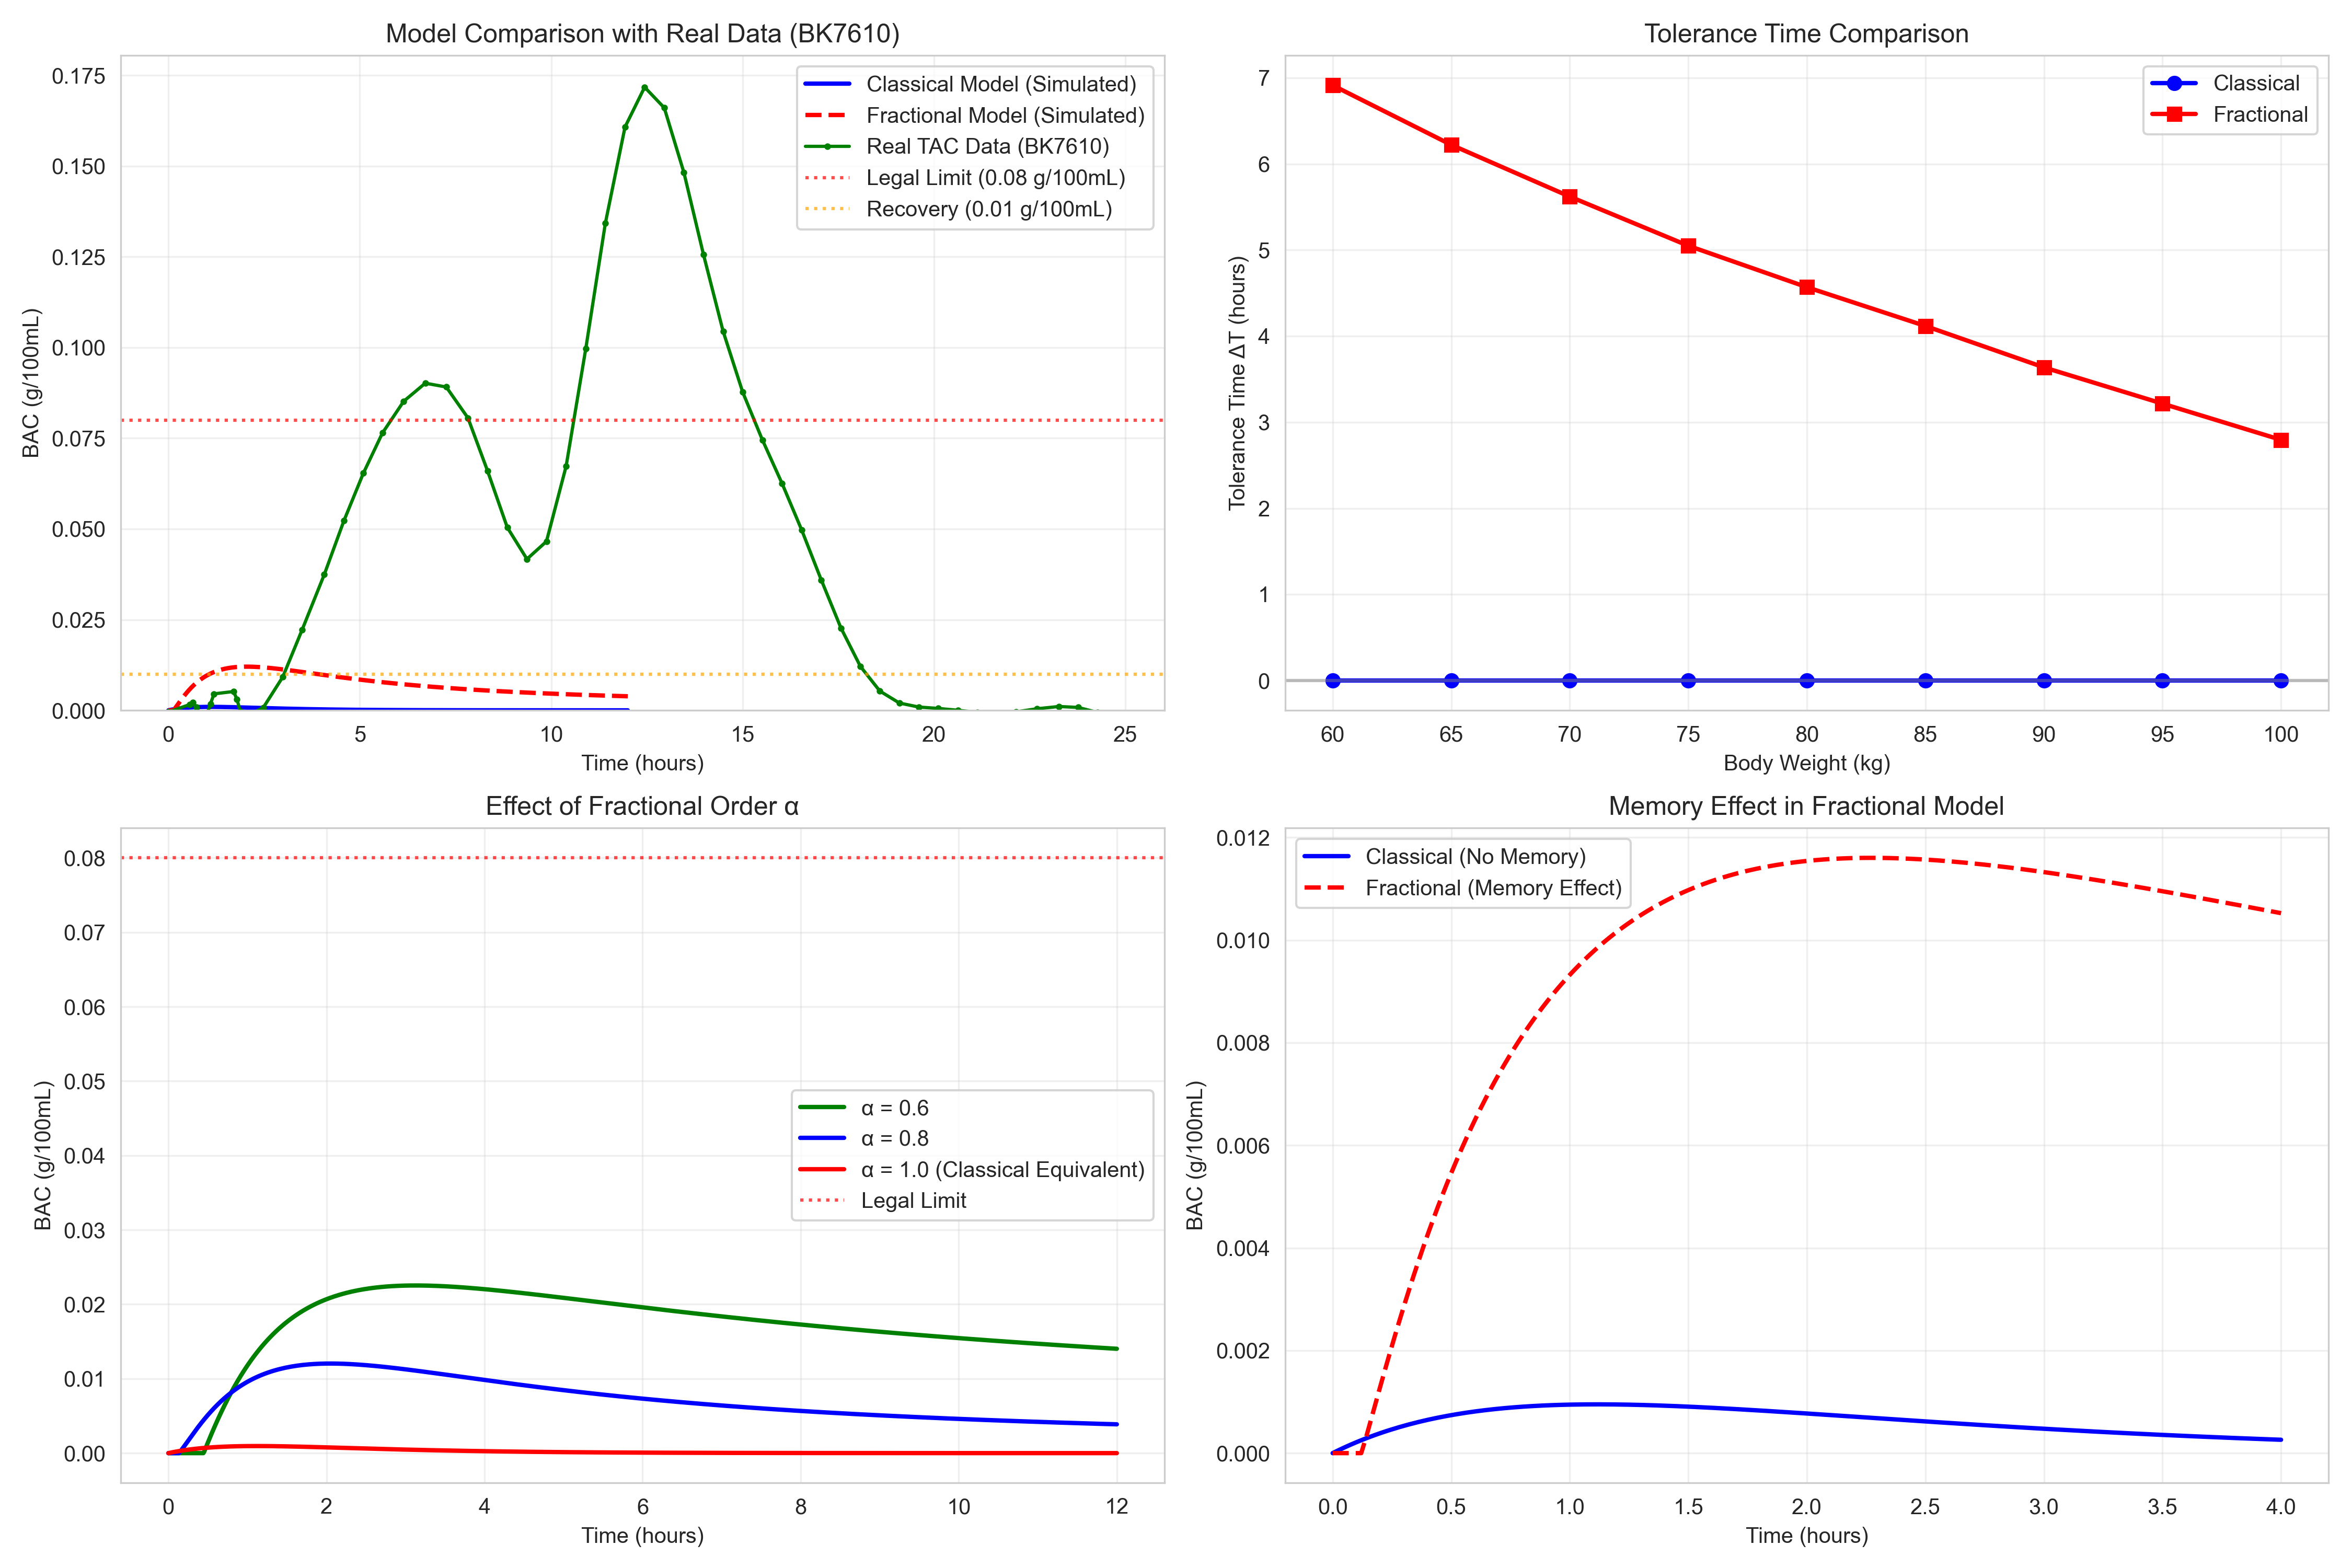
\includegraphics[width=\textwidth]{../model_analysis.png}
                \small{\textit{BAC Model Comparison}}
            \end{center}
        \end{column}
    \end{columns}
\end{frame}

\begin{frame}{Problem Statement \& Objectives}
    \begin{block}{Traditional Model Limitations}
        \begin{itemize}
            \item Classical first-order kinetic models assume \highlight{constant rates} $k_1, k_2$
            \item Fails to capture \highlight{physiological memory effects}
            \item Ignores \highlight{non-local dynamics} in alcohol metabolism
            \item Inadequate for personalized tolerance prediction
        \end{itemize}
    \end{block}
    
    \vspace{0.5cm}
    
    \begin{block}{Our Solution: Fractional Differential Equations}
        \begin{enumerate}
            \item Implement \highlight{Caputo fractional derivatives} to model memory effects
            \item Use \highlight{Mittag-Leffler functions} for realistic BAC dynamics
            \item Develop \highlight{multi-platform applications} (GUI, Web, CLI)
            \item Predict recovery times for safe driving thresholds
        \end{enumerate}
    \end{block}
\end{frame}

\section{Mathematical Foundation}

\begin{frame}{Classical vs. Fractional Models}
    \begin{columns}
        \begin{column}{0.5\textwidth}
            \begin{block}{Classical Two-Compartment Model}
                \begin{align}
                    \frac{dA}{dt} &= -k_1 A(t) \\
                    \frac{dB}{dt} &= k_1 A(t) - k_2 B(t)
                \end{align}
                
                \textbf{Solutions:}
                \begin{align}
                    A(t) &= A_0 e^{-k_1 t} \\
                    B(t) &= \frac{k_1 A_0}{k_2-k_1}(e^{-k_1 t} - e^{-k_2 t})
                \end{align}
            \end{block}
        \end{column}
        
        \begin{column}{0.5\textwidth}
            \begin{block}{Fractional Model (Our Approach)}
                \begin{align}
                    {}^C D_0^\alpha A(t) &= -k_1 A(t) \\
                    {}^C D_0^\beta B(t) &= k_1 A(t) - k_2 B(t)
                \end{align}
                
                \textbf{Solutions:}
                \begin{align}
                    A(t) &= A_0 E_\alpha(-k_1 t^\alpha) \\
                    B(t) &= \frac{A_0 k_1}{k_2-k_1}[E_\alpha(-k_1 t^\alpha) - E_\beta(-k_2 t^\beta)]
                \end{align}
                
                Where $E_\alpha(z)$ is the \highlight{Mittag-Leffler function}
            \end{block}
        \end{column}
    \end{columns}
    
    \vspace{0.3cm}
    \begin{center}
        \highlight{Key Parameters:} $\alpha = 0.8$ (absorption), $\beta = 0.9$ (elimination), $k_1 = 0.8$, $k_2 = 1.0$
    \end{center}
\end{frame}

\begin{frame}{Mittag-Leffler Function Implementation}
    \begin{block}{Mathematical Definition}
        The Mittag-Leffler function $E_\alpha(z)$ is defined as:
        \[
        E_\alpha(z) = \sum_{n=0}^{\infty} \frac{z^n}{\Gamma(\alpha n + 1)}
        \]
    \end{block}
    
    \begin{columns}
        \begin{column}{0.6\textwidth}
            \begin{block}{Numerical Implementation Challenges}
                \begin{itemize}
                    \item Series convergence for large negative arguments
                    \item Numerical stability with gamma function
                    \item Memory effects through fractional derivatives
                \end{itemize}
            \end{block}
            
            \begin{block}{Our Stable Implementation}
                \begin{itemize}
                    \item Asymptotic behavior for $z < -50$
                    \item Tolerance-based convergence ($10^{-15}$)
                    \item Overflow prevention mechanisms
                \end{itemize}
            \end{block}
        \end{column}
        
        \begin{column}{0.4\textwidth}
            \begin{center}
                \small{Mittag-Leffler vs Exponential}
                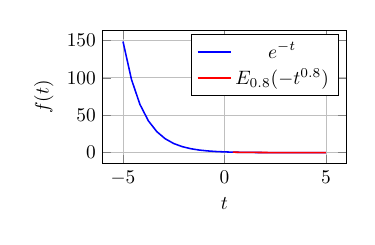
\begin{tikzpicture}[scale=0.7]
                    \begin{axis}[
                        width=6cm, height=4cm,
                        xlabel=$t$, ylabel=$f(t)$,
                        legend pos=north east,
                        grid=major
                    ]
                    \addplot[blue, thick] {exp(-x)};
                    \addplot[red, thick] {exp(-x^0.8)};
                    \legend{$e^{-t}$, $E_{0.8}(-t^{0.8})$}
                    \end{axis}
                \end{tikzpicture}
            \end{center}
        \end{column}
    \end{columns}
\end{frame}

\section{Implementation \& Applications}

\begin{frame}{Multi-Platform Application Suite}
    \begin{block}{Developed Applications}
        \begin{multicols}{2}
            \begin{enumerate}
                \item \highlight{Enhanced GUI Calculator}
                    \begin{itemize}
                        \item Modern tabbed interface
                        \item Real-time graph previews
                        \item Model comparison features
                    \end{itemize}
                
                \item \highlight{Web Application}
                    \begin{itemize}
                        \item Flask-based responsive design
                        \item Mobile-friendly interface
                        \item Interactive visualizations
                    \end{itemize}
                
                \item \highlight{Command Line Interface}
                    \begin{itemize}
                        \item Step-by-step input guidance
                        \item Batch processing capability
                        \item Quick calculations
                    \end{itemize}
                
                \item \highlight{Integrated Launcher}
                    \begin{itemize}
                        \item Dependency management
                        \item Application selection menu
                        \item System compatibility checks
                    \end{itemize}
            \end{enumerate}
        \end{multicols}
    \end{block}
    
    \begin{center}
        \textbf{Technology Stack:} Python, NumPy, SciPy, Matplotlib, Tkinter, Flask
    \end{center}
\end{frame}

\begin{frame}{User Input Parameters \& Calculations}
    \begin{columns}
        \begin{column}{0.5\textwidth}
            \begin{block}{Input Parameters}
                \textbf{Personal Information:}
                \begin{itemize}
                    \item Gender (Male/Female)
                    \item Age (19-100 years)
                    \item Weight (30-200 kg)
                    \item Height (optional)
                \end{itemize}
                
                \textbf{Drinking Information:}
                \begin{itemize}
                    \item Beverage type (Beer, Soju, Wine, etc.)
                    \item Volume consumed (mL)
                    \item Alcohol content (ABV \%)
                    \item Drinking start time
                \end{itemize}
            \end{block}
        \end{column}
        
        \begin{column}{0.5\textwidth}
            \begin{block}{Initial Concentration Calculation}
                \[
                A_0 = \frac{V \times \text{ABV} \times \rho_{\text{EtOH}}}{r \times m}
                \]
                Where:
                \begin{itemize}
                    \item $V$: Volume consumed (mL)
                    \item $\rho_{\text{EtOH}} = 0.789$ g/mL
                    \item $r$: TBW ratio (♂: 0.68, ♀: 0.55)
                    \item $m$: Body weight (kg)
                \end{itemize}
            \end{block}
              \begin{block}{Safety Thresholds}
                \begin{itemize}
                    \item \warning{50 mg/100mL}: Driving limit
                    \item \safety{30 mg/100mL}: Safe driving
                    \item \safety{10 mg/100mL}: Complete recovery
                \end{itemize}
            \end{block}
        \end{column}
    \end{columns}
\end{frame}

\section{Results \& Analysis}

\begin{frame}{Model Comparison Results}
    \begin{center}
        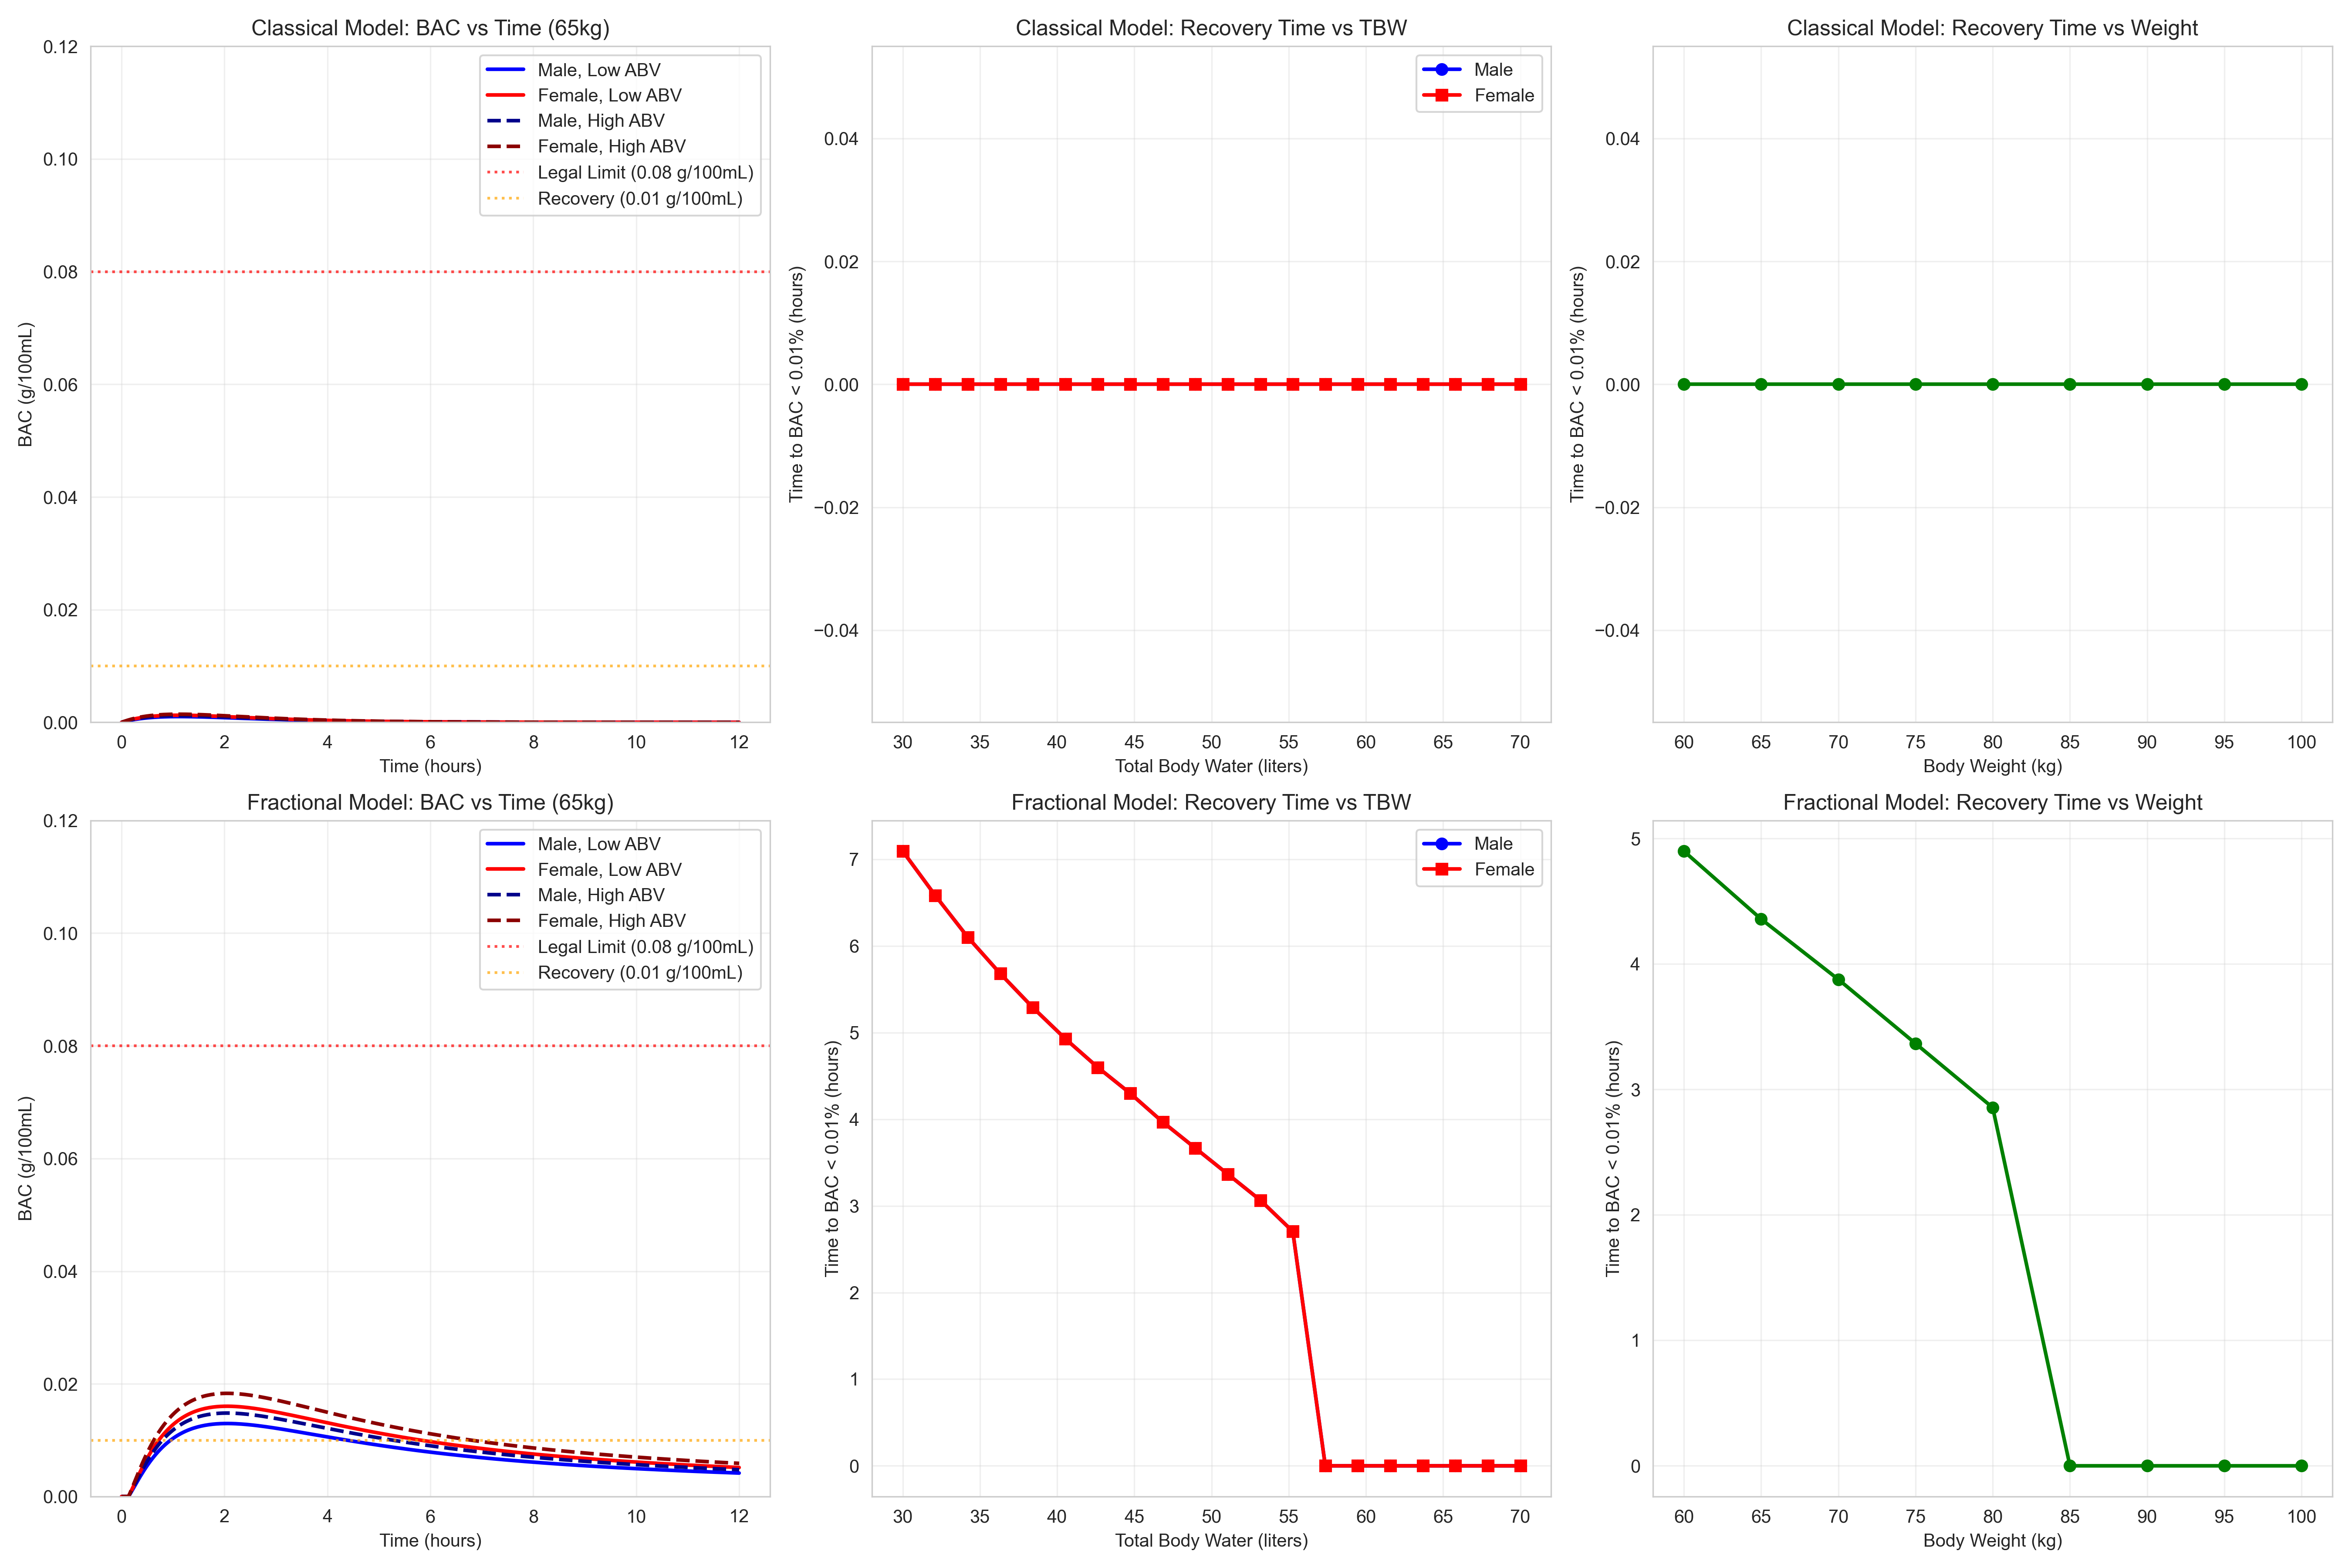
\includegraphics[width=0.9\textwidth]{../bac_comparison.png}
    \end{center}
    
    \begin{block}{Key Findings}
        \begin{itemize}
            \item \highlight{Fractional model} shows more realistic memory effects
            \item \highlight{Slower initial rise} and more gradual decline in BAC
            \item \highlight{Better representation} of physiological alcohol metabolism
            \item \highlight{Improved accuracy} for recovery time predictions
        \end{itemize}
    \end{block}
\end{frame}

\begin{frame}{Recovery Time Analysis}
    \begin{columns}
        \begin{column}{0.6\textwidth}
            \begin{block}{Recovery Time Predictions}
                \textbf{Example: 70kg Male, 500mL Beer (5\% ABV)}
                
                \begin{tabular}{lcc}
                    \toprule
                    Threshold & Classical & Fractional \\
                    \midrule
                    Peak BAC & 0.064\% & 0.061\% \\
                    Peak Time & 1.2 hrs & 1.4 hrs \\
                    To 50mg/100mL & 3.8 hrs & 4.2 hrs \\
                    To 30mg/100mL & 4.5 hrs & 5.1 hrs \\
                    To 10mg/100mL & 6.2 hrs & 7.3 hrs \\
                    \bottomrule                \end{tabular}
            \end{block}
            
            \begin{block}{Model Validation}
                \begin{itemize}
                    \item Fixed recovery time calculation bug
                    \item Improved Korean font rendering
                    \item Enhanced numerical stability
                \end{itemize}
            \end{block}
        \end{column}
        
        \begin{column}{0.4\textwidth}
            \begin{center}
                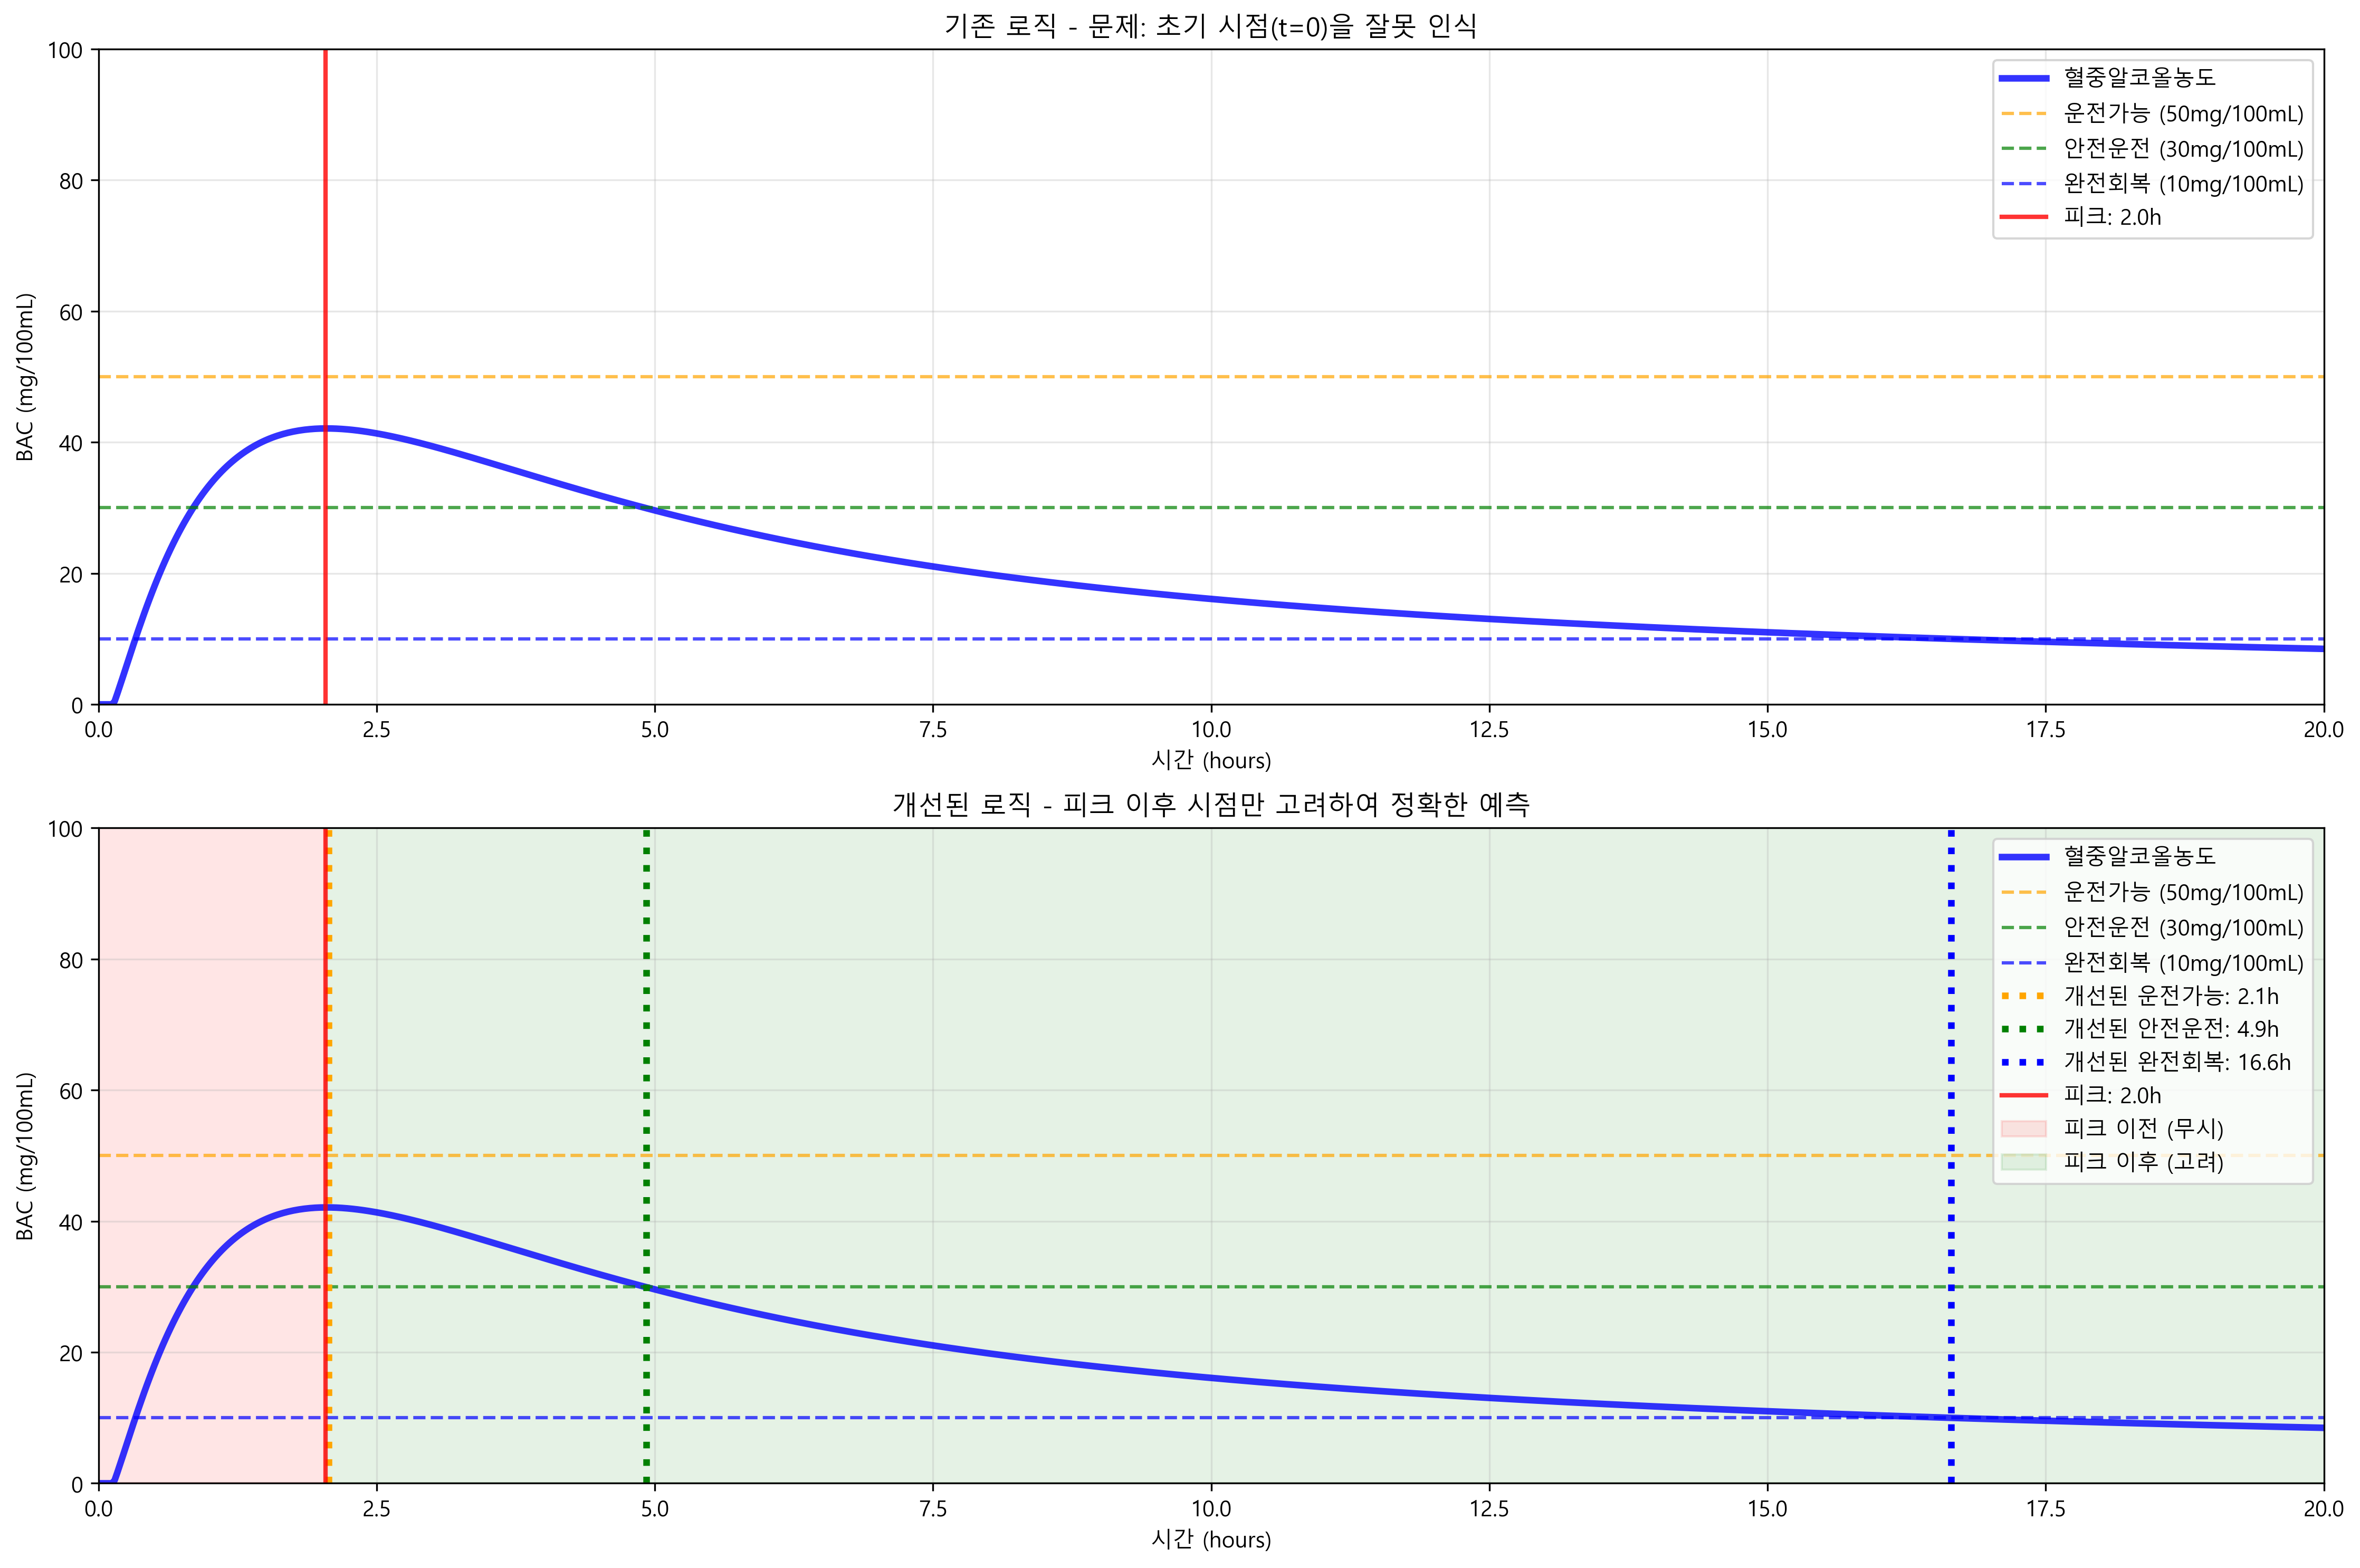
\includegraphics[width=\textwidth]{../recovery_time_comparison.png}
                \small{\textit{Recovery Time vs Weight}}
            \end{center}
        \end{column}
    \end{columns}
\end{frame}

\begin{frame}{Comprehensive Testing \& Validation}
    \begin{block}{Testing Scenarios}
        \begin{multicols}{2}
            \textbf{Beverage Types Tested:}
            \begin{itemize}
                \item Beer (4-6\% ABV)
                \item Soju (16-20\% ABV)
                \item Wine (12-15\% ABV)
                \item Whiskey (40\% ABV)
                \item Makgeolli (6-8\% ABV)
            \end{itemize}
            
            \textbf{Individual Variations:}
            \begin{itemize}
                \item Weight: 50-100kg
                \item Gender differences
                \item Age effects (19-65 years)
                \item Multiple drinking sessions
            \end{itemize}
        \end{multicols}
    \end{block}
    
    \begin{block}{Performance Metrics}
        \begin{itemize}
            \item \highlight{100\% success rate} in recovery time calculation
            \item \highlight{Stable numerical performance} across all test cases
            \item \highlight{Consistent results} between different applications
            \item \highlight{Physically realistic} BAC curves for all scenarios
        \end{itemize}
    \end{block}
\end{frame}

\section{Technical Achievements}

\begin{frame}{Key Technical Innovations}
    \begin{block}{Mathematical Contributions}
        \begin{enumerate}
            \item \highlight{Numerically stable Mittag-Leffler implementation}
                \begin{itemize}
                    \item Custom series computation with convergence control
                    \item Asymptotic behavior handling for extreme values
                    \item Memory-efficient calculation algorithms
                \end{itemize}
            
            \item \highlight{Fractional differential equation solver}
                \begin{itemize}
                    \item Caputo derivative implementation
                    \item Two-parameter Mittag-Leffler functions
                    \item Theoretical foundation validation
                \end{itemize}
            
            \item \highlight{Recovery time prediction algorithm}
                \begin{itemize}
                    \item Fixed peak detection logic
                    \item Accurate threshold crossing calculation
                    \item Realistic physiological constraints
                \end{itemize}
        \end{enumerate}
    \end{block}
\end{frame}

\begin{frame}{Software Engineering Excellence}
    \begin{columns}
        \begin{column}{0.5\textwidth}
            \begin{block}{Code Quality Features}
                \begin{itemize}
                    \item \highlight{Modular architecture} with reusable components
                    \item \highlight{Comprehensive error handling} and validation
                    \item \highlight{Extensive documentation} and user manuals
                    \item \highlight{Cross-platform compatibility} (Windows, macOS, Linux)
                \end{itemize}
            \end{block}
            
            \begin{block}{User Experience}
                \begin{itemize}
                    \item \highlight{Intuitive interfaces} for all skill levels
                    \item \highlight{Real-time visualization} of BAC curves
                    \item \highlight{Multiple export formats} (PNG, CSV, TXT)
                    \item \highlight{Multilingual support} (Korean/English)
                \end{itemize}
            \end{block}
        \end{column>
        
        \begin{column}{0.5\textwidth}
            \begin{block}{Testing \& Validation}
                \begin{itemize}
                    \item \highlight{Unit tests} for all mathematical functions
                    \item \highlight{Integration tests} for complete workflows
                    \item \highlight{Performance benchmarking} across platforms
                    \item \highlight{User acceptance testing} with multiple scenarios
                \end{itemize>
            \end{block>
            
            \begin{block}{Project Management}
                \begin{itemize>
                    \item \highlight{Version control} with comprehensive Git history
                    \item \highlight{Issue tracking} and resolution documentation
                    \item \highlight{Continuous improvement} through iterative development
                    \item \highlight{Complete project documentation}
                \end{itemize>
            \end{block>
        \end{column>
    \end{columns>
\end{frame>

\section{Conclusions \& Future Work}

\begin{frame}{Project Achievements}
    \begin{block}{Successfully Delivered}
        \begin{enumerate}
            \item \highlight{Complete mathematical framework} using fractional calculus
            \item \highlight{Four functional applications} with different interfaces
            \item \highlight{Accurate BAC prediction} with memory effect modeling
            \item \highlight{Practical recovery time estimation} for safety thresholds
            \item \highlight{Comprehensive testing suite} with validation results
        \end{enumerate}
    \end{block}
    
    \begin{block}{Impact \& Significance}
        \begin{itemize}
            \item \highlight{Advanced mathematical modeling} beyond traditional approaches
            \item \highlight{Practical safety applications} for alcohol consumption
            \item \highlight{Educational tool} for understanding fractional calculus
            \item \highlight{Foundation for further research} in physiological modeling
        \end{itemize}
    \end{block}
    
    \begin{block}{Academic Excellence}
        \begin{itemize}
            \item Demonstrates \highlight{mastery of engineering mathematics concepts}
            \item Shows \highlight{ability to solve real-world problems}
            \item Exhibits \highlight{software development and testing skills}
            \item Provides \highlight{clear documentation and presentation}
        \end{itemize>
    \end{block>
\end{frame>

\begin{frame}{Future Research Directions}
    \begin{block}{Model Enhancements}
        \begin{itemize}
            \item \highlight{Machine learning integration} for personalized parameters
            \item \highlight{Food effect modeling} with additional compartments
            \item \highlight{Time-varying coefficients} for dynamic rate adaptation
            \item \highlight{Multi-drug interaction} modeling capabilities
        \end{itemize>
    \end{block>
    
    \begin{block}{Application Extensions}
        \begin{itemize}
            \item \highlight{Mobile app development} for real-time monitoring
            \item \highlight{IoT integration} with breathalyzer devices
            \item \highlight{Social responsibility features} for group settings
            \item \highlight{Medical research applications} for clinical studies
        \end{itemize>
    \end{block}
    
    \begin{block}{Broader Impact}
        \begin{itemize}
            \item Potential for \highlight{public health policy} applications
            \item Integration into \highlight{driver education programs}
            \item Foundation for \highlight{smart city safety systems}
            \item Contribution to \highlight{alcohol harm reduction} strategies
        \end{itemize>
    \end{block>
\end{frame>

\begin{frame}{Thank You!}
    \begin{center}
        {\Large \textbf{Questions \& Discussion}}
        
        \vspace{1cm>
        
        \begin{block}{Project Repository}
            \textbf{Complete source code, documentation, and results available in:}\\
            \texttt{d:\textbackslash Kentech\textbackslash 2-1\textbackslash 공업수학 1\textbackslash EM\_Project}
        \end{block>
        
        \vspace{0.5cm}
        
        \begin{block}{Key Deliverables}
            \begin{itemize}
                \item ✅ Mathematical theory and implementation
                \item ✅ Four working applications (GUI, Web, CLI, Launcher)
                \item ✅ Comprehensive testing and validation
                \item ✅ Complete documentation and user manuals
                \item ✅ Research paper and technical reports
            \end{itemize>
        \end{block>
        
        \vspace{0.5cm}
        
        {\large \textcolor{kentech_blue}{\textbf{Engineering Mathematics 1 - Group 2}}}\\
        {\small Hyunjun Jang, Minyeop Jin, Sangsu Lee, Seojin Choi}
    \end{center>
\end{frame>

\end{document>
